\documentclass[10pt]{article}

\linespread{1} 
\usepackage{float}

\usepackage{geometry}
 \geometry{
  papersize={175mm,248mm},
 total={175mm,248mm},
 left=26mm,
 right=13mm,
 bottom=17mm,
 top=13mm,
 }


\usepackage{amsfonts,amssymb,graphicx,color,epstopdf}
\usepackage[font=small,labelfont=bf]{caption}
\usepackage{subcaption}

\usepackage{color, colortbl, framed}
\usepackage[T1]{fontenc}
\usepackage{mathptmx}

\usepackage{amsmath}
%\usepackage{lineno,hyperref}
\usepackage{authblk}
\usepackage{titlesec}
\usepackage{eucal}
%\DeclareMathAlphabet{\mathpzc}{OT1}{pzc}{m}{it}
%\usepackage{epstopdf}

\usepackage{hhline}
\usepackage{xcolor,colortbl}
\renewcommand{\figurename}{Fig.}

%  \setcounter{secnumdepth}{0}
\usepackage{titlesec}
\titlespacing{\section}{0pt}{\parskip}{-\parskip}
\titlespacing{\subsection}{0pt}{\parskip}{-\parskip}
 \titleformat*{\section}{\normalfont\fontfamily{ptm}\fontsize{10}{19}\bfseries}
 \titleformat*{\subsection}{\normalfont\fontfamily{ptm}\fontsize{10}{18}\bfseries}


\usepackage[sort&compress,square]{natbib}
\setlength{\bibsep}{0.0pt}


\usepackage{authblk}
\usepackage{varwidth}

\renewcommand*{\Authsep}{, }
\renewcommand*{\Authand}{, }
\renewcommand*{\Authands}{, }
\renewcommand*{\Affilfont}{\normalsize\normalfont}
\renewcommand*{\Authfont}{\normalsize\normalfont\bfseries}
\setlength{\affilsep}{0em}

\renewcommand{\abstractname}{}    % clear the title
\makeatletter
\renewcommand{\maketitle}{\bgroup\setlength{\parindent}{0pt}
\begin{flushleft}
  \textbf{\@title}
\vspace{10pt}

  \@author
\end{flushleft}\egroup
}
\makeatother

\title{\fontsize{16pt}{10pt}\selectfont\flushleft \textbf{Informative frequency band identification for automatic extraction of impulsive components in vibration data from rotating machinery}}
% \author{}
\author[1]{Jacek Wodecki}
\author[2]{Rados{\l}aw Zimroz}
\author[3]{Tomasz Barszcz}
% \author[2]{Agnieszka Wy{\l}oma{\'n}ska}


\affil[1,2]{Faculty of Geoengineering, Mining and Geology, Wroclaw University of Science and Technology, Na Grobli 15, 50-421 Wroclaw, Poland}
\affil[3]{AGH University of Science and Technology, Krakow, Poland
\protect\\
\textbf{E-mail:} $^{1}${jacek.wodecki@pwr.edu.pl},$^{2}${radoslaw.zimroz@pwr.edu.pl},\protect\\ $^{3}${tbarszcz@agh.edu.pl}}


\date{} 

\begin{document}
\maketitle
\textbf{Abstract.}In this paper authors address the issue of local damage detection in rolling element bearings in the presence of non-Gaussian noise. Typically damage detection problems concern the techniques of filtration, decomposition, separation, extraction etc. In such real-life cases main difficulty lies in non-Gausianity of the noise present in the operational environment, hence popular denoising techniques cannot be used. In presented article a real-life industrial scenario will be discussed and a new approach to cyclic component extraction will be presented. Classical detection methods are often not sufficient for the task because of high energy of impulsive noise in comparison to spectral structure of the damage. Proposed method utilizes Cyclic Spectral Coherence map as two-dimensional data representation, and Nonnegative Matrix Factorization as analytical tool to extract individual components.
\newline \newline
\textbf{Keywords:} vibration analysis, damage detection,  rolling element bearings, cyclostationarity analysis, nonnegative matrix factorization.

\section{Introduction}

Identification and diagnostics of damage in rotating machines is still an open subject. For such kind of analysis the most frequently used medium is vibration signal. In case of local damage, faults like cracks, pitting or breakage manifest themselves in the vibration signal as cyclic, impulsive and typically nonstationary components. It is critical to detect such anomalies in early stage of damage evolution to avoid unexpected and costly stoppages in the future. From the perspective of signal processing, the problem comes down to identification of impulsive component buried in wideband stationary background, that can consist of Gaussian noise and deterministic components, for example meshing components for gearboxes \cite{randall2011rolling}. 

In general vibration signal needs to be preprocessed to extract so-called Signal of Interest (SOI). Such preprocessing can be performed using techniques such as bandpass filtering, wavelet decomposition \cite{lin2003gearbox}, adaptive filtering \cite{makowski2014new}, statistical modeling \cite{zak2014application,nowicka2006dependence}, time-frequency analysis \cite{wodecki2016combination} or cyclostationary analysis \cite{boustany2005subspace,kruczek2017cyclic}. Unfortunately, in case of real-life industrial signals such classical methods of diagnostic analysis are prone to insufficient effectiveness. It is necessary to introduce specialized multidimensional representations of the data that are able to tackle the issue of frequency-related analysis. In relation to such representations, it is required to incorporate specialized analytical techniques that can extract information in a different way. 

In presented paper authors reach for the bi-frequency representation called Cyclic Spectral Coherence map (CSC), that can reveal modulation spectra related to different carrier frequencies. To analyze such representation, Nonnegative Matrix Factorization (NMF) is used for differentiation of spectra that are connected to different processes occurring within the signal \cite{wang2013nonnegative,lee1999learning,he2011symmetric}. 

\section{Object of interest}

The studied machine is a gas compressor of a type Dresser Rand C-VIP, that has been already studied by Barszcz et al. \cite{barszcz2013bearings}. The key issue is that vibration signals generated by the compressor contain a number of external disturbances, the most influential being the piston-related and valve related ones. It has been discovered that the analyzed signal has been recorded when the bearing inner ring has been severely defected in one of the main shaft bearings. Details including the SOI parameters are presented in Table \ref{tab:tab1}. 

\begin{table}[ht!]
    \centering
    \caption{Machine-related frequencies}
    \begin{tabular}{|l|l|}
    \hline
         \textbf{Parameter} & \textbf{Frequency [Hz]} \\ \hline
         Sampling frequency & 24000 \\ \hline
         Shaft speed & 12.35 \\ \hline
         BPFI & 127.9 \\ 
    \hline
    \end{tabular}
    \label{tab:tab1}
\end{table}

Impulses at the rate of approximately 12.35 Hz are observable. They reveal themselves directly on the DFT spectrum, dominating its low-frequency part (up to about 3 kHz), while the further part of the spectrum appears to be a noise-like behavior. Since the 12.35 Hz is the rotational speed, it is obvious that the main impulsive component is piston and valve-related. Bearing fault related impacts are not detectable on the spectrum.

\section{Methodology}

\begin{figure}[h!]
\centering
\includegraphics[width=0.35\textwidth]{wykresy/block}
\caption{Flowchart of proposed procedure}
\label{fig:block}
\end{figure}

In this section the presented methodology is described. Firstly Cyclic Spectral Coherence map is calculated for raw input data, which is then provided to Nonnegative Matrix Factorization algorithm for selector bank definition. When selectors are defined, they are used as ordinary filters used to filter the original signal. Filtration with each of the filters outputs one of the signal components. General flowchart of the procedure is presented in Fig. \ref{fig:block}.

\subsection{Cyclic Spectral Coherence}

In signals coming from rotating machinery for each carrier frequency different modulation frequencies can arise. Hence, bi-frequency method should be used in such analysis. In order to describe this effect Antoni in 2007 introduced the spectral coherence (SC) \cite{antoni2007cyclic}. Let us remind the cyclic power spectrum (CPS) $S_X(f;\alpha)$ of the signal $\mathbf{x}$:

\begin{equation}
\label{eq:CPS}
S_X(f;\alpha)=\lim_{L\to \infty} \frac{1}{L}\mathbb{E} \left(\mathcal{F}_{\mathbf{x},L} (f+\frac{\alpha}{2})\overline{\mathcal{F}_{\mathbf{x},L}(f-\frac{\alpha}{2})}\right),
\end{equation}

where $\mathcal{F}_{\mathbf{x},L}(f)$ is Fourier transform of the signal $\mathbf{x}$ calculated on interval of length $L$. According to equation~(\ref{eq:CPS}) the CPS describes dependence of the spectral components being apart by given modulation frequency $\alpha$ for carrier frequency $f$. Obviously, the cyclostationary signal is expected to reveal $\left|S_X(f;\alpha)\right|>0$ for modulation frequency $\alpha\neq 0$. Given the definition of CPS, the formula for SC can be defined ~\cite{antoni2007cyclic}:

\begin{equation}
\label{eq:SC}
\left|\gamma_X(f;\alpha)\right|^{2}=\frac { \left|S_X(f;\alpha)\right|^2 }{ S_X(f+\frac{\alpha}{2};0)S_X(f-\frac{\alpha}{2};0)}.
\end{equation}

Obtained statistic is normalized. Therefore, SC quantifies the spectral cyclic autocorrelation of the signal. Indeed, when $\left|\gamma_X(f;\alpha)\right|^{2}$ is close to one then signal reveals the cyclostationarity property at carrier frequency f with modulation period equal to $T=1/\alpha$ .
According to equation~(\ref{eq:SC}) the estimation of SC can be directly performed with estimator of CPS. Namely, the estimator of SC is given by formula:

\begin{equation}
\left|\hat{\gamma}_X(f;\alpha)\right|^{2}=\frac{ \left|\hat{S}_X(f;\alpha)\right|^2 
}{\hat{S}_X(f+\frac{\alpha}{2};0)\hat{S}_X(f-\frac{\alpha}{2};0)},
\end{equation} 

where $\hat{S}_X(f;\alpha)$ is an estimator of the CPS.

\subsection{NMF}
Nonnegative Matrix Factorization has been selected as separation method. Thanks to general inherent clustering properties of NMF-type algorithms such method can be used to aggregate different types of behavior within the analyzed matrix into separate classes. Presented methodology uses classic NMF with Euclidean objective function and multiplicative update rule \cite{wodecki2017local}.

\section{Application to real data}

Fig. \ref{fig:raw} illustrates a short section of vibration measurement that has been used for analysis. As a first step, CSC map has been calculated for full Nyquist range and up to 300 Hz of modulating frequency, with the 128-sample Hamming window, 110-sample overlap and 256 FFT points (see Fig. \ref{fig:csc}).


\begin{figure}[h!]
\centering
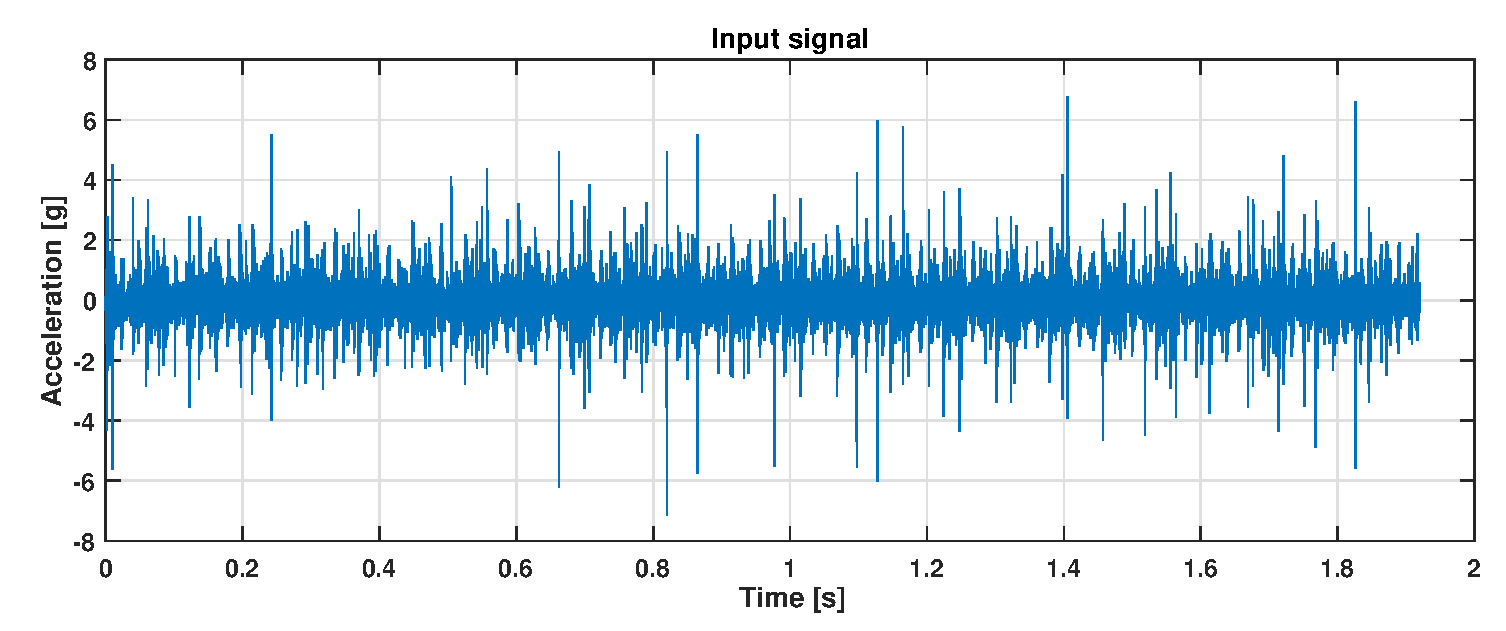
\includegraphics[width=0.9\textwidth]{wykresy/raw}
\caption{Raw vibration data}
\label{fig:raw}
\end{figure}

After that the map has been provided to NMF algorithm that recognized different spectral signatures of the desired components (see Fig. \ref{fig:trans}). 

\begin{figure}[h!]
\centering
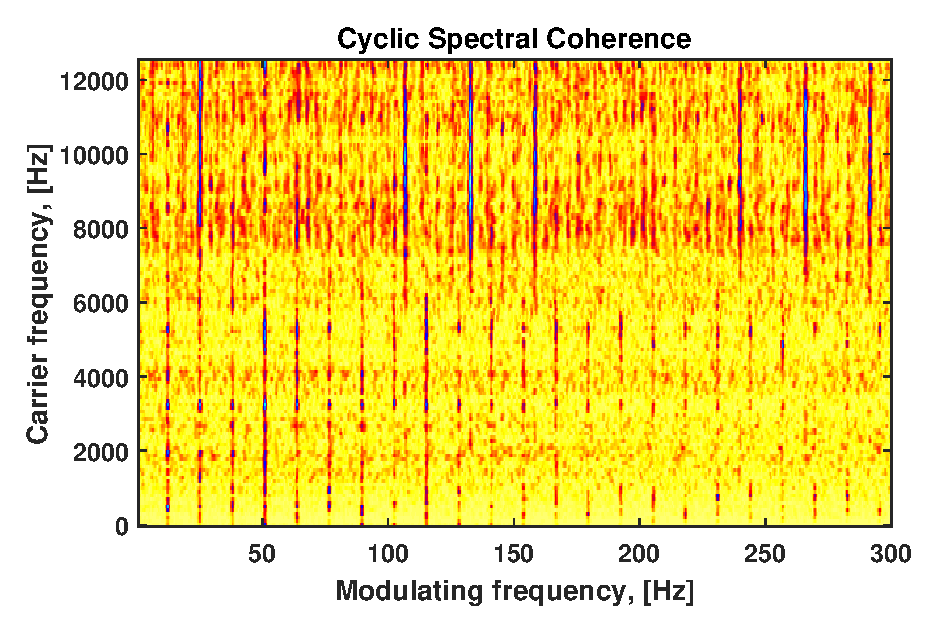
\includegraphics[width=0.7\textwidth]{wykresy/csc}
\caption{Cyclic Spectral Coherence map}
\label{fig:csc}
\end{figure}

\begin{figure}[h!]
\centering
\includegraphics[width=\textwidth]{wykresy/trans.png}
\caption{Construction of filter bank using NMF base matrix}
\label{fig:trans}
\end{figure}

Input signal has been then filtered with both of the spectral signatures to produce two output signals, each dominantly carrying one of regarded cyclic components.

\begin{figure}[h!]
\centering
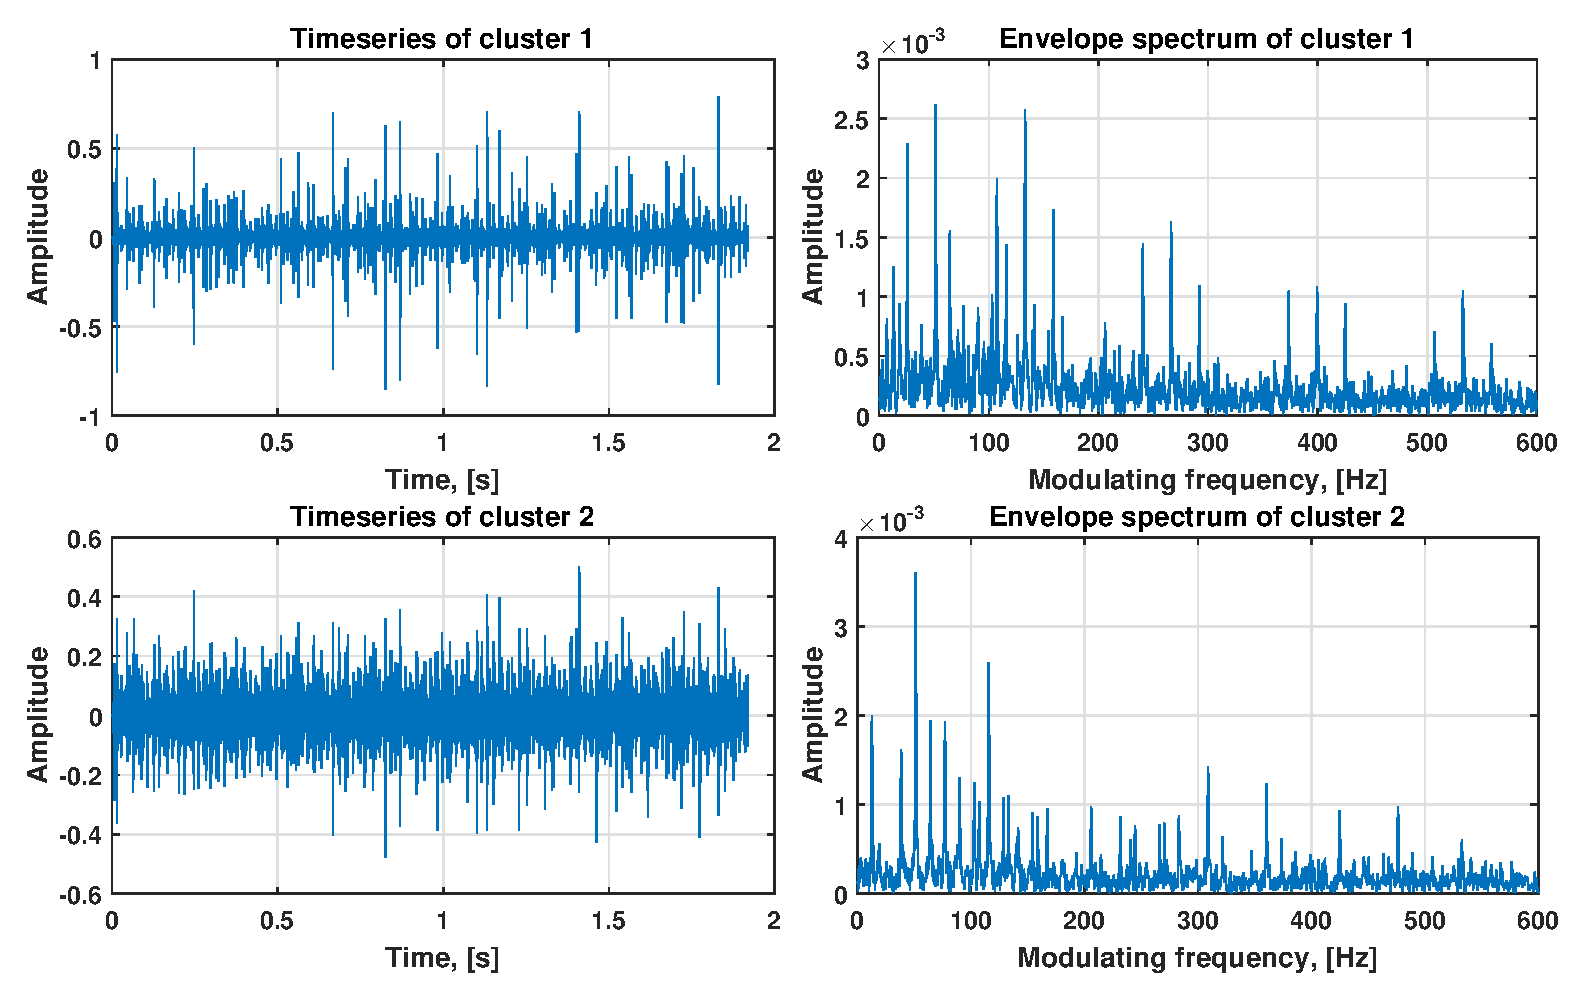
\includegraphics[width=\textwidth]{wykresy/out}
\caption{Results of method operation. Left panels: extracted time series, right panels: corresponding envelope spectra.}
\label{fig:out}
\end{figure}

While time series of obtained components reveal impulsive components much more clearly than the original signal (Fig. \ref{fig:out} left panels), their regarded periodicity is most pronounced in the envelope modulation spectra (Fig. \ref{fig:out} right panels). First cluster reveals desired information about bearing fault cycle recognized as 127.8 Hz for the fundamental modulating frequency, and second cluster presents expected shaft cycle with fundamental modulating frequency recognized as 12.45 Hz, which corresponds perfectly with theoretical frequencies calculated based on machine kinematics, down to FFT sample precision.

\section{Conclusions}

In presented article authors focused on the problem of fault frequency component identification in vibration data from gas compressor. Cyclic Spectral Density map is used as multidimensional signal representation, and it is used for informative frequency band identification performed further by classic Nonnegative Matrix Factorization algorithm. One of the matrices provided by NMF, called base matrix, is used as a filter bank for raw signal filtration. In opposition to classical methods of frequency or time-frequency analysis, presented algorithm was able to pinpoint the fault frequency connected to the bearing operation, which was difficult to recognize in the original signal. Further research will be focused on enhancing the performance of NMF algorithm by algebraic preprocessing of the CSC map, that is expected to improve the conditioning properties of spectral signatures distinction.

\bibliographystyle{JVE_style}
\bibliography{mybibfile}

\end{document}